\chapter{Laboratorio 3: \\Clock gating, pipelining and parallelizing}
Durante questa esperienza di laboratorio verranno analizzate una serie di tecniche per ridurre i consumi mediante l'ottimizzazione dell'architettura dei circuiti.
\section{A first approach to clock gating}
Un prima tecnica utilizzata per ridurre i consumi andando a lavorare sull'architettura è il \textit{Clock Gating}. Questa tecnica permette di "staccare" il clock ad un determinato blocco del mio circuito, quando questo non deve lavorare. Un circuito di massima è riportato in Figura \ref{clock_gating}. \\
\begin{figure}[!htb]
	\centering
	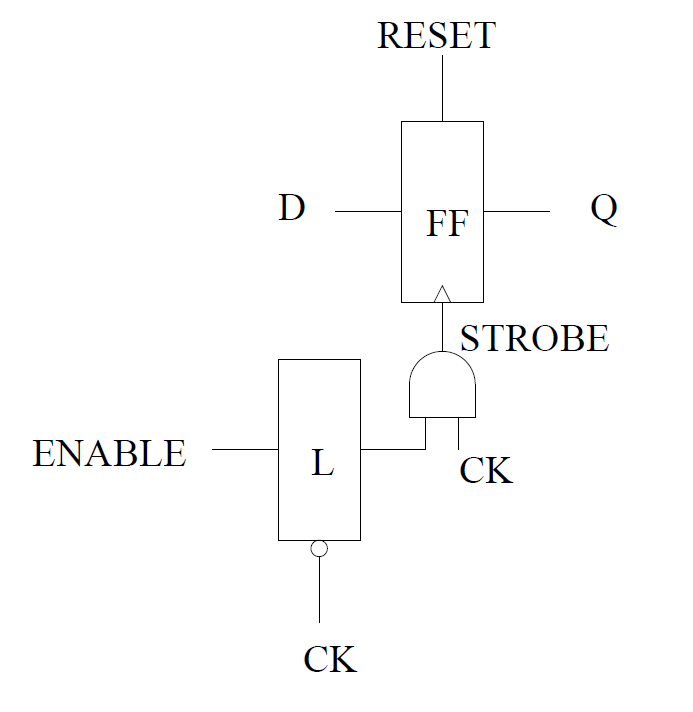
\includegraphics[scale=0.60]{immagini/clock_gating}
	\caption{\textit{Schema implementativo della tecnica del Clock Gating}}
	\label{clock_gating}
\end{figure}
\newpage
\noindent Nella prima parte dell'esperienza viene chiesto di analizzare il file \textit{ckgbug.vhd} che contiene la descrizione VHDL di una struttura composta da due registri in cascata, denominati L1 ed L2. La tecnica del clock gating viene applicata al secondo registro, mediante una AND tra il clock e un segnale di ENABLE. \\
Bisogna prestare attenzione al fatto che i segnali di ingresso dei due registri (D1 e D2) siano rispettivamente \textit{std\_logic\_vector (7 downto 0)} e \textit{std\_logic\_vector (0 to 7}. \\
In una prima simulazione, si forza il segnale D1 al valore '01111111' e, attivando il segnale di ENABLE, ci si aspetterebbe che D2, al colpo di clock successivo, vada al valore '111111101' e che l'uscita di L2, denominata D3, vada al valore '01111111' al colpo di clock ancora successivo. In realtà la simulazione porta al risultato in Figura \ref{clock_gat1}.
\begin{figure}[!htb]
	\centering
	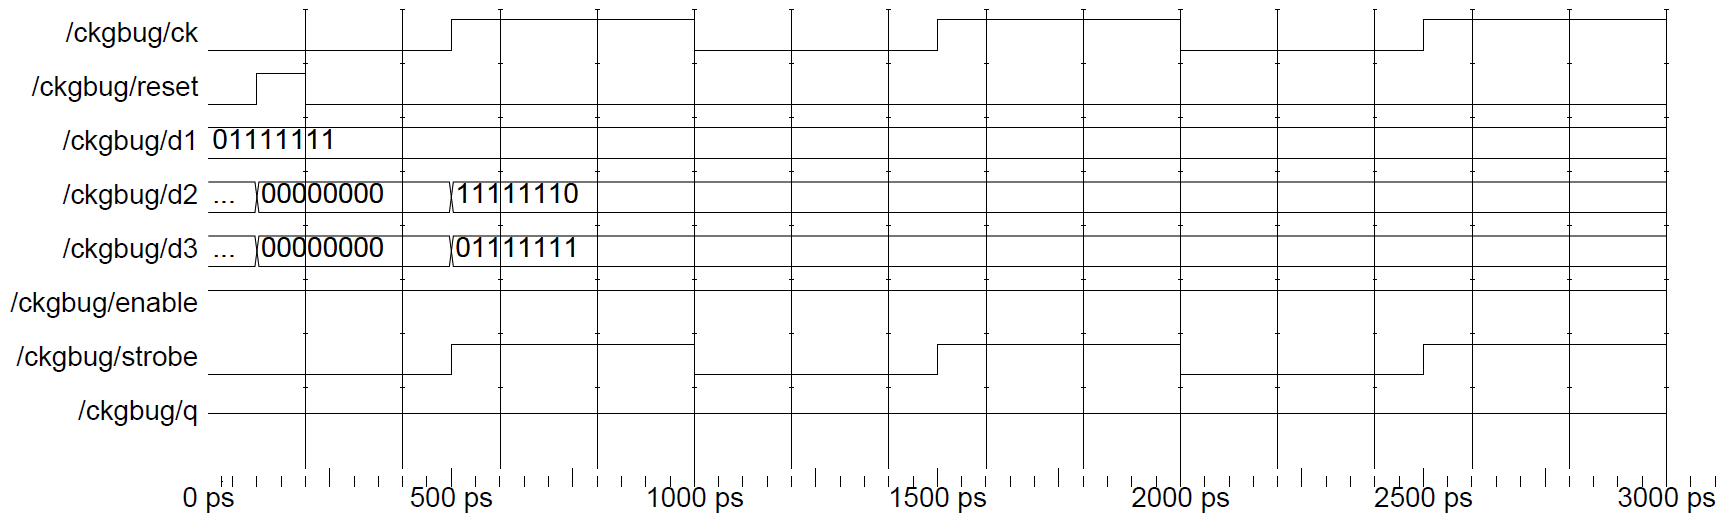
\includegraphics[scale=0.8]{immagini/clock_gating1}
	\caption{\textit{Schema implementativo della tecnica del Clock Gating}}
	\label{clock_gat1}
\end{figure}
Si può ben notare come l'uscita D3 dopi esattamente D1 dopo un solo colpo di clock. Questo è dovuto al fatto che il clock gated arriva a L2 un "passo di simulazione" dopo L1, perchè il simulatore programma il calcolo dell'uscita AND dopo l'assegnazione del clock. Quindi accade come se l'AND avesse un ritardo interno. \\
La traccia suggerisce che si può risolvere questo inconveniente andando ad aggiungere un ritardo \textit{Clock-to-Output} pari a 0.1 ps all'uscita del generico Flip-Flop. Andando a risimulare il file, si ottiene il comportamento desiderato, che viene riportato in Figura \ref{clock_gat2}. \\
\newpage
\begin{figure}[!htb]
	\centering
	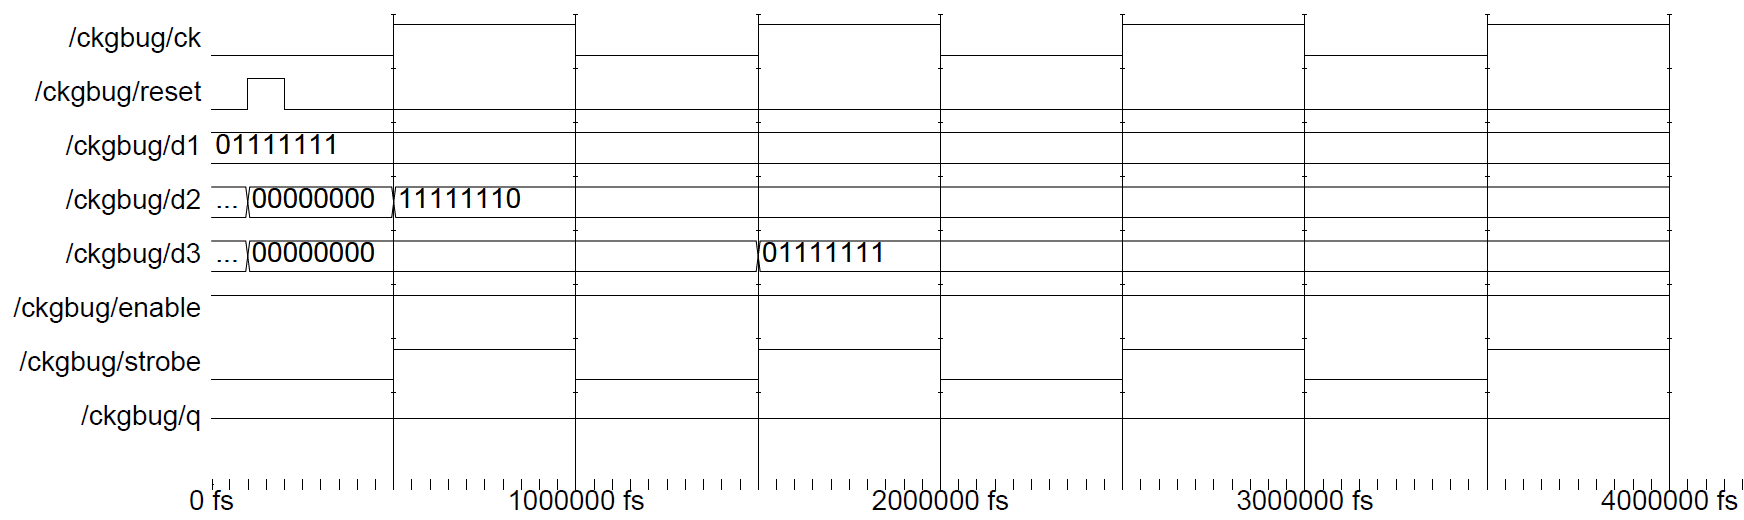
\includegraphics[scale=0.8]{immagini/clock_gating2}
	\caption{\textit{Schema implementativo della tecnica del Clock Gating}}
	\label{clock_gat2}
\end{figure}
\noindent Infine si aggiunge un ulteriore ritardo alla porta AND pari a 0.2 ps, ossia un tempo superiore a quello \textit{Clock-to-Output} inserito in precendeza. In questo modo si va a violtare il $t_{hold}$ e dunque il circuito ritorna nella situazione precendete con un funzionamento non corretto. Il risultato della simulazione è riportato in Figura \ref{clock_gat3}. \\
\begin{figure}[!htb]
	\centering
	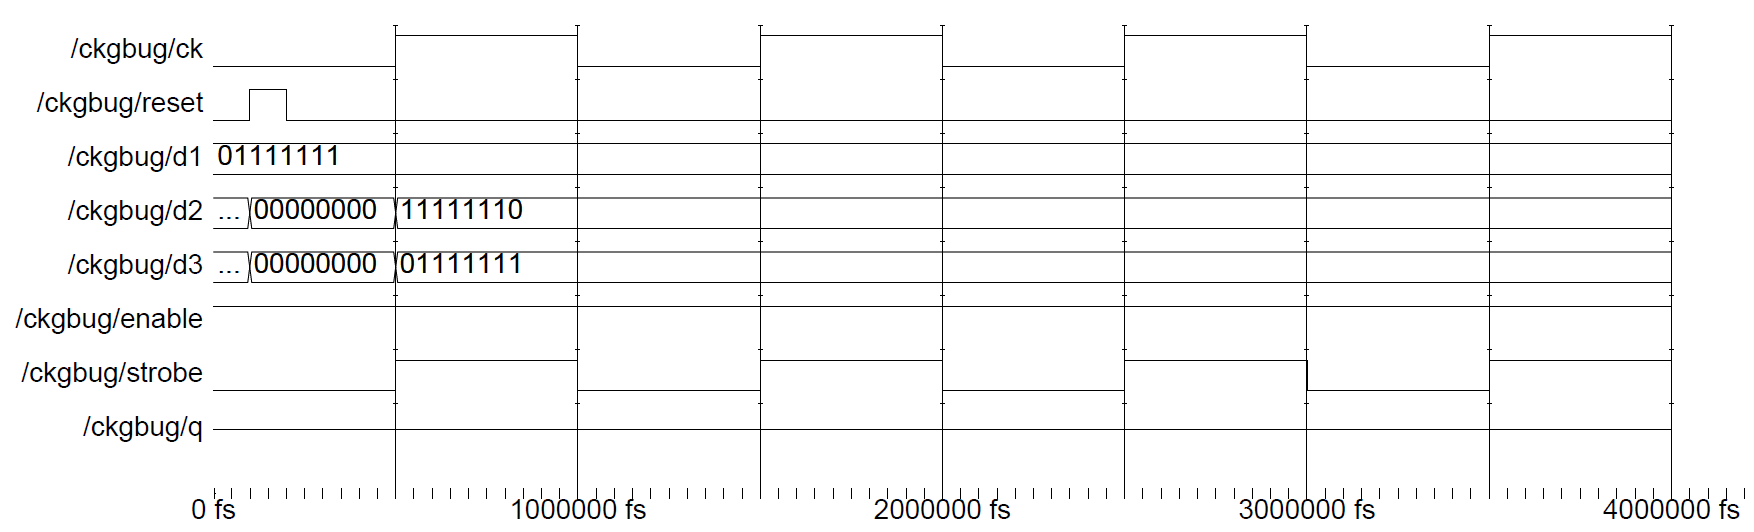
\includegraphics[scale=0.8]{immagini/clock_gating3}
	\caption{\textit{Schema implementativo della tecnica del Clock Gating}}
	\label{clock_gat3}
\end{figure}

\section{Clock Gating for a complex circuit}